\section{Dinamica}

\subsection{Principi fondamentali}

\begin{center}
    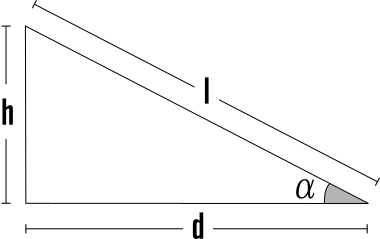
\includegraphics[width=0.6\linewidth]{Dinamica/piano-inclinato-senza-angolo.png} \\    
\end{center}

\begin{gather*}
    \begin{cases}
        \sin \alpha = \frac{h}{l} \\ 
        \cos \alpha = \frac{d}{l} \\
        \tan \alpha = \frac{h}{d} \\
    \end{cases} \rightarrow 
    \begin{cases}
        h = l \cdot \sin \alpha \\
        l = \frac{h}{\sin \alpha}
    \end{cases} \\
    \text{Secondo principio: } \\
    \vec{F} = m \vec{a} \\
    \vec{a} = \frac{\vec{F}}{m} \\
    m = \frac{\vec{F}}{a} \\
    \text{Terzo principio: } \vec{F}_{AB} = -\vec{F}_{BA}
\end{gather*}
\subsection{Piano inclinato}
\begin{gather*}
    F_{P, x} = F_P \sin (\alpha) = m g \sin (\alpha) \\
    F_{P, y} = F_P \cos (\alpha) = m g \cos (\alpha) 
\end{gather*}
%%%
\subsubsection{Piano inclinato senza attrito}
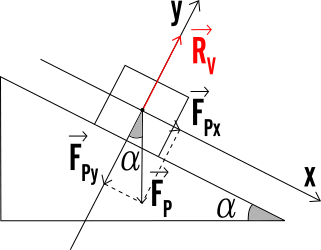
\includegraphics[width=0.75 \linewidth]{Dinamica/reazione-vincolare-nel-piano-inclinato.png} \\
\begin{gather*}
\textbf{Accelerazione}: \begin{cases}
    a_y = 0 \\
    a_x = g \sin{\alpha}
\end{cases}
\end{gather*}

\subsubsection{Piano inclinato con F verso l'alto}
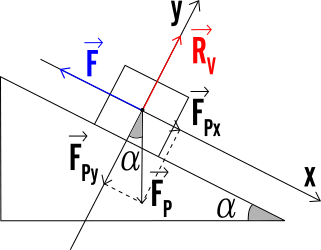
\includegraphics[width=0.75 \linewidth]{Dinamica/variante-piano-inclinato-senza-attrito.png} \\
\textbf{Nota bene: } sull'asse y la forza($F$)che spinge l'oggetto verso l'alto non fa cambiare niente. Ricordiamo che abbiamo scelto \textbf{il piano inclinato} come asse del nostro sistema di riferimento.
\begin{gather*}
    \text{Forza risultante: } F_{ris} = F_{P, x} - F \\
    \text{Accelerazione: } a = \frac{F_{ris}}{m} \\
    \begin{cases}
        F_{P, x} > F & \text{Corpo scende, $a$ positiva} \\
        F_{P, x} < F & \text{Corpo sale, $a$ negativa}
    \end{cases}
\end{gather*}
%%%
\subsubsection{Piano inclinato con attrito}
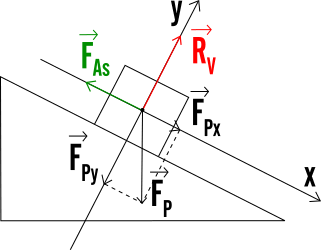
\includegraphics[width=0.75 \linewidth]{Dinamica/piano-inclinato-con-attrito.png} \\
\begin{gather*}
    \textbf{Forza risultante: } F_{ris, x} = \sqrt{F_{P, x}^2 + F_{As}^2}
\end{gather*}
\textbf{Nota bene: } la forza d'attrito ($F_{A}$, attrito statico nell'immagine) ha verso opposto alla componente della forza peso sull'asse x($F_{P, x}$)
\subsubsection{Piano inclinato con attrito e forza aggiuntiva}
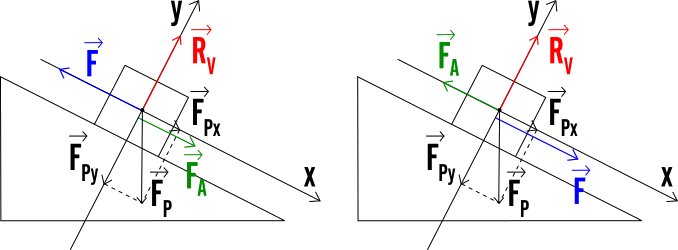
\includegraphics[width=\linewidth]{Dinamica/piano-inclinato-con-attrito-2.png} \\
\textbf{Primo caso: } forza risultante($F_{ris, x}$)tutta concentrata lungo l'asse $x$: $F_{ris, x} = F - F_A - F_{P, x}$ \\
\textbf{Secondo caso: } $F_{ris, x} = F + F_{P, x} - F_A$ \\

\subsubsection{Attrito Statico}
\begin{gather*}
    \textbf{Forza Attrito Statico: } \\ F_{As} = \mu_s \cdot F_\perp = \mu_s \cdot F_{P, y} = \mu_s m g \cos (\alpha) \\
    \textbf{Accelerazione: } \\ a = a_x = g \sin (\alpha) - \mu_s g \cos (\alpha) \\
    \textbf{Angolo critico per l'equilibrio: } \\ \alpha = \arctan (\mu_s) : \\
    \begin{cases}
        \text{Scivola} & \text{Angoli } > \alpha \\
        \text{Equilibrio} & \text{Angoli } <= \alpha
    \end{cases}    \\
    \textbf{Attrito Statico per Equilibrio: } \mu_s = \tan (\alpha)
\end{gather*}
\textbf{Nota bene: } affinché una macchina(su terreno piano, $\cos (\alpha) = 0$) non slitti, la Forza di Attrito Statico($F_{As}$) deve essere uguale alla Forza($\vec{F}$) che la macchina esegue per andare avanti, quindi: $F_{As} = F \rightarrow \mu_s m g = m a \rightarrow \mu_s = \frac{a}{g}$
\subsubsection{Attrito Dinamico}
\textbf{Nota bene: } Per poter considerare il problema dal punto di vista dell'attrito dinamico($\mu_d$) il corpo deve essere già in movimento!
\begin{gather*}
    \textbf{Forza Attrito Dinamico:} \\ F_{Ad} = \mu_d \cdot F_\perp = \mu_d \cdot F_{P, y} = \mu_d m g \cos (\alpha) \\
    \textbf{Accelerazione: } \\ a = a_x = g \sin (\alpha) - \mu_d g \cos (\alpha)
\end{gather*}

\subsection{Molle e Forza Elastica}
\begin{center}
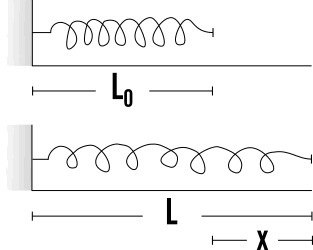
\includegraphics[width=0.4 \linewidth]{Dinamica/forza-elastica.png} 
\end{center}
\begin{gather*}
    \text{Lunghezza della molla a riposo: } L_0 \\
    \text{Elongazione: } x = L - L_0 \\
    \text{Legge di Hooke(Forza Elastica): } F_e = -k x
\end{gather*}
\subsection{Forza Centripeta}
\textbf{Nota bene: } possiamo ricondurci alla forza centripeta($F_c$) usando le formule per la forza($F = m \cdot a$) e l'accelerazione centripeta($a_c = \frac{v^2}{r} = \omega^2 \cdot r $)! Utilizziamo queste formule per problemi come \textbf{macchine in un circuito di raggio $r$ e coefficiente di attrito dinamico $\mu_d$ dove non deve slittare}.
\\
\begin{gather*}
    \text{Forza centripeta: } F_c = m \frac{v^2}{r} cos (\alpha) \\
    \text{Forza centripeta: } F_c = m \cdot \omega^2 \cdot r
\end{gather*}

\textbf{Nota bene: } se vogliamo che un corpo rimanga nella sua traiettoria circolare, allora la la forza di accelerazione($F_a$)deve essere uguale alla forza centripeta($F_c$).

\begin{center}
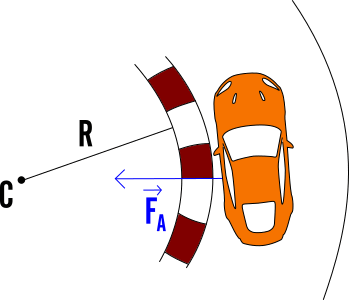
\includegraphics[width=0.7 \linewidth]
{Dinamica/forza-centripeta.png}
\end{center}
\begin{gather*}
    \text{Equivalenza: } F_a = F_c \rightarrow \mu_d  g = \frac{v^2}{r} \\
    \text{Coefficiente d'attrito minimo: } \mu = \frac{v^2}{g \cdot r} \\
    \text{Velocità minima: } v = \sqrt{\mu_d \cdot g \cdot r}
\end{gather*}
\subsection{Lavoro}

\textbf{Nota bene: } il lavoro($F$) è energia trasferita ad un corpo mediante le forze che agiscono su di esso. \\
\begin{center}
    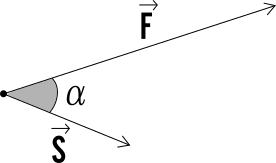
\includegraphics[width=0.4 \linewidth]{Dinamica/Lavoro./il-lavoro-di-una-forza.png}    
\end{center}
\begin{gather*}
    \textbf{Lavoro: } L = \vec{F} \cdot \vec{s} = F \cdot  s
\end{gather*}

\subsection{Lavoro della forza peso}

\begin{gather*}
    \textbf{Lavoro: } L = -mg(y_{finale} - y_{iniziale})
\end{gather*}

\subsection{Lavoro della forza elastica}

\begin{gather*}
    \textbf{Lavoro: } L = - \frac{1}{2} k (x_f^2 - x_i^2) \\
    \textbf{Elongazione iniziale: } x_i = L_i - L_0 \\
    \textbf{Elongazione finale: } x_f = L_f - L_0
\end{gather*}

\textbf{Nota bene: } nel caso di una molla a riposo($x_i = 0$)il lavoro($L$) sarà sempre negativo, che la molla venga compressa($x_f < 0$) o che venga allungata($x_f > 0$), poiché la forza elastica della molla resiste all'elongazione.

\begin{gather*}
    \textbf{Molla compressa: } x_f < 0 \\
    \textbf{Molla allungata: } x_f > 0 \\
    \textbf{Lavoro: } L = - \frac{1}{2} k (x_f^2)
\end{gather*}
\subsection{Energia}
\textbf{Nota bene: } l'energia è una grandezza che esprime la capacità di un corpo/sistema di compiere un lavoro, indipendentemente dal fatto che il lavoro venga compiuto o meno. Si divide in: \textit{cinetica, potenziale, meccanica}.

\subsection{Energia Cinetica}

\begin{gather*}
    \text{Teorema Energia Cinetica: } L = \Delta K \\
    \text{Energia Cinetica: } K = \frac{1}{2} m v^2 \\
    \text{Massa: } m = \frac{2K}{v^2} \\
    \text{Velocità: } v = \sqrt{\frac{2K}{m}} \\
    \text{Variazione Energia Cinetica: } \\ \Delta K = K_f - K_i = \frac{1}{2} m v_f^2 - \frac{1}{2} m v_i^2
\end{gather*}

\subsection{Oscillatore armonico(Pendolo)}
\begin{gather*}
    \textbf{Frequenza: } T = 2 \pi \sqrt{\frac{l}{a_g}} \\
    \textbf{Lunghezza Pendolo: } l = \frac{g T^2}{4 \pi^2} \\
    \textbf{Accelerazione gravitazionale: } \\ a_g = \frac{M \cdot G}{r_{distanza}^2}
\end{gather*}